\documentclass{semdoc}
% Template: $Id: t01_txt.tex,v 1.7 2000/05/23 12:13:37 bless Exp $
% -----------------------------------------------------------------------------
%epstopdf ermöglicht, dass eps-Dateien durch pdflatex in windows eingebunden werden können
%\usepackage{epstopdf}
% Report Praktikum
% -----------------------------------------------------------------------------
% Kommentare beginnen mit einem %-Zeichen
\docbegin
% --> Oberhalb der Linie bitte nichts ändern.
% ---------------------------------------------------------------------------
% \/ \/ \/ \/ \/ \/ \/ \/ \/ \/ \/ \/ \/ \/ \/ \/ \/ \/ \/ \/ \/ \/ \/ \/ \/
% Stellen, an denen etwas geaendert werden soll, sind wie hier gekennzeichnet.
% /\ /\ /\ /\ /\ /\ /\ /\ /\ /\ /\ /\ /\ /\ /\ /\ /\ /\ /\ /\ /\ /\ /\ /\ /\

%
% ---------------------------------------------------------------------------
% \/ \/ \/ \/ \/ \/ \/ \/ \/ \/ \/ \/ \/ \/ \/ \/ \/ \/ \/ \/ \/ \/ \/ \/ \/
% --> Bitte den Titel des Beitrages in die nächste Zeile eintragen:
\title{Praktikumsbericht 5}
%
% --> ... und den Namen des Autors:
\author{Jean-Marc Hendrikse}
% /\ /\ /\ /\ /\ /\ /\ /\ /\ /\ /\ /\ /\ /\ /\ /\ /\ /\ /\ /\ /\ /\ /\ /\ /\
% -----------------------------------------------------------------------------

% Nicht ändern!
\event{Access Control Systems Lab\\}
\term{Sommersemester 2017}
\supervisor{Prof. Dr. Hannes Hartenstein, Alexander Degitz, Jan Grashöfer, Till Neudecker}

%
%
\maketitle

\section*{Einleitung} % in die Klammern die Ueberschrift
\label{Introduction} % und ein Label

Die Attributbasierte Zugriffskontrolle (Attribute-Based Access Control, ABAC) kommt ursprünglich aus dem Umfeld der Service-Orientierten Architekturen. Mithilfe von ABAC ist es möglich Ausdrücke über Attribute von Benutzern, Ressource und Umgebung zu definieren.

\section{Azure Zugriffsrechte}
In diesem Kapitel wird beschrieben wie die Azure Zugriffsrechte funktionieren und wie die Zugriffskontrolle auf Ressourcen anhand von Testbenutzern, die versuchen auf Ressourcen zuzugreifen, erfolgt.  Als Testbenutzer dienen uns die aus der letzten Praktikumsaufgabe erstellten Benutzer: Test1, Test2 und Test3. Zusätzlich definieren wir 2 Gruppen: Group Testgroup12, zu der Test1 und Test2 gehören, und Testgroup13, in der Test1 und Test3 zugeordnet sind.\\
Initial befinden sich keine zugewiesenen Ressourcen zum Testen für die Benutzer im Azure Portal.\\
Über All Ressources > DC – Access control (IAM) > Add permission können neue Rollen den Benutzern zugeordnet werden, die in einem bestimmten Scope agieren dürfen. Siehe Grafik \ref{res}
\\
\begin{figure}[h]
    \centering
    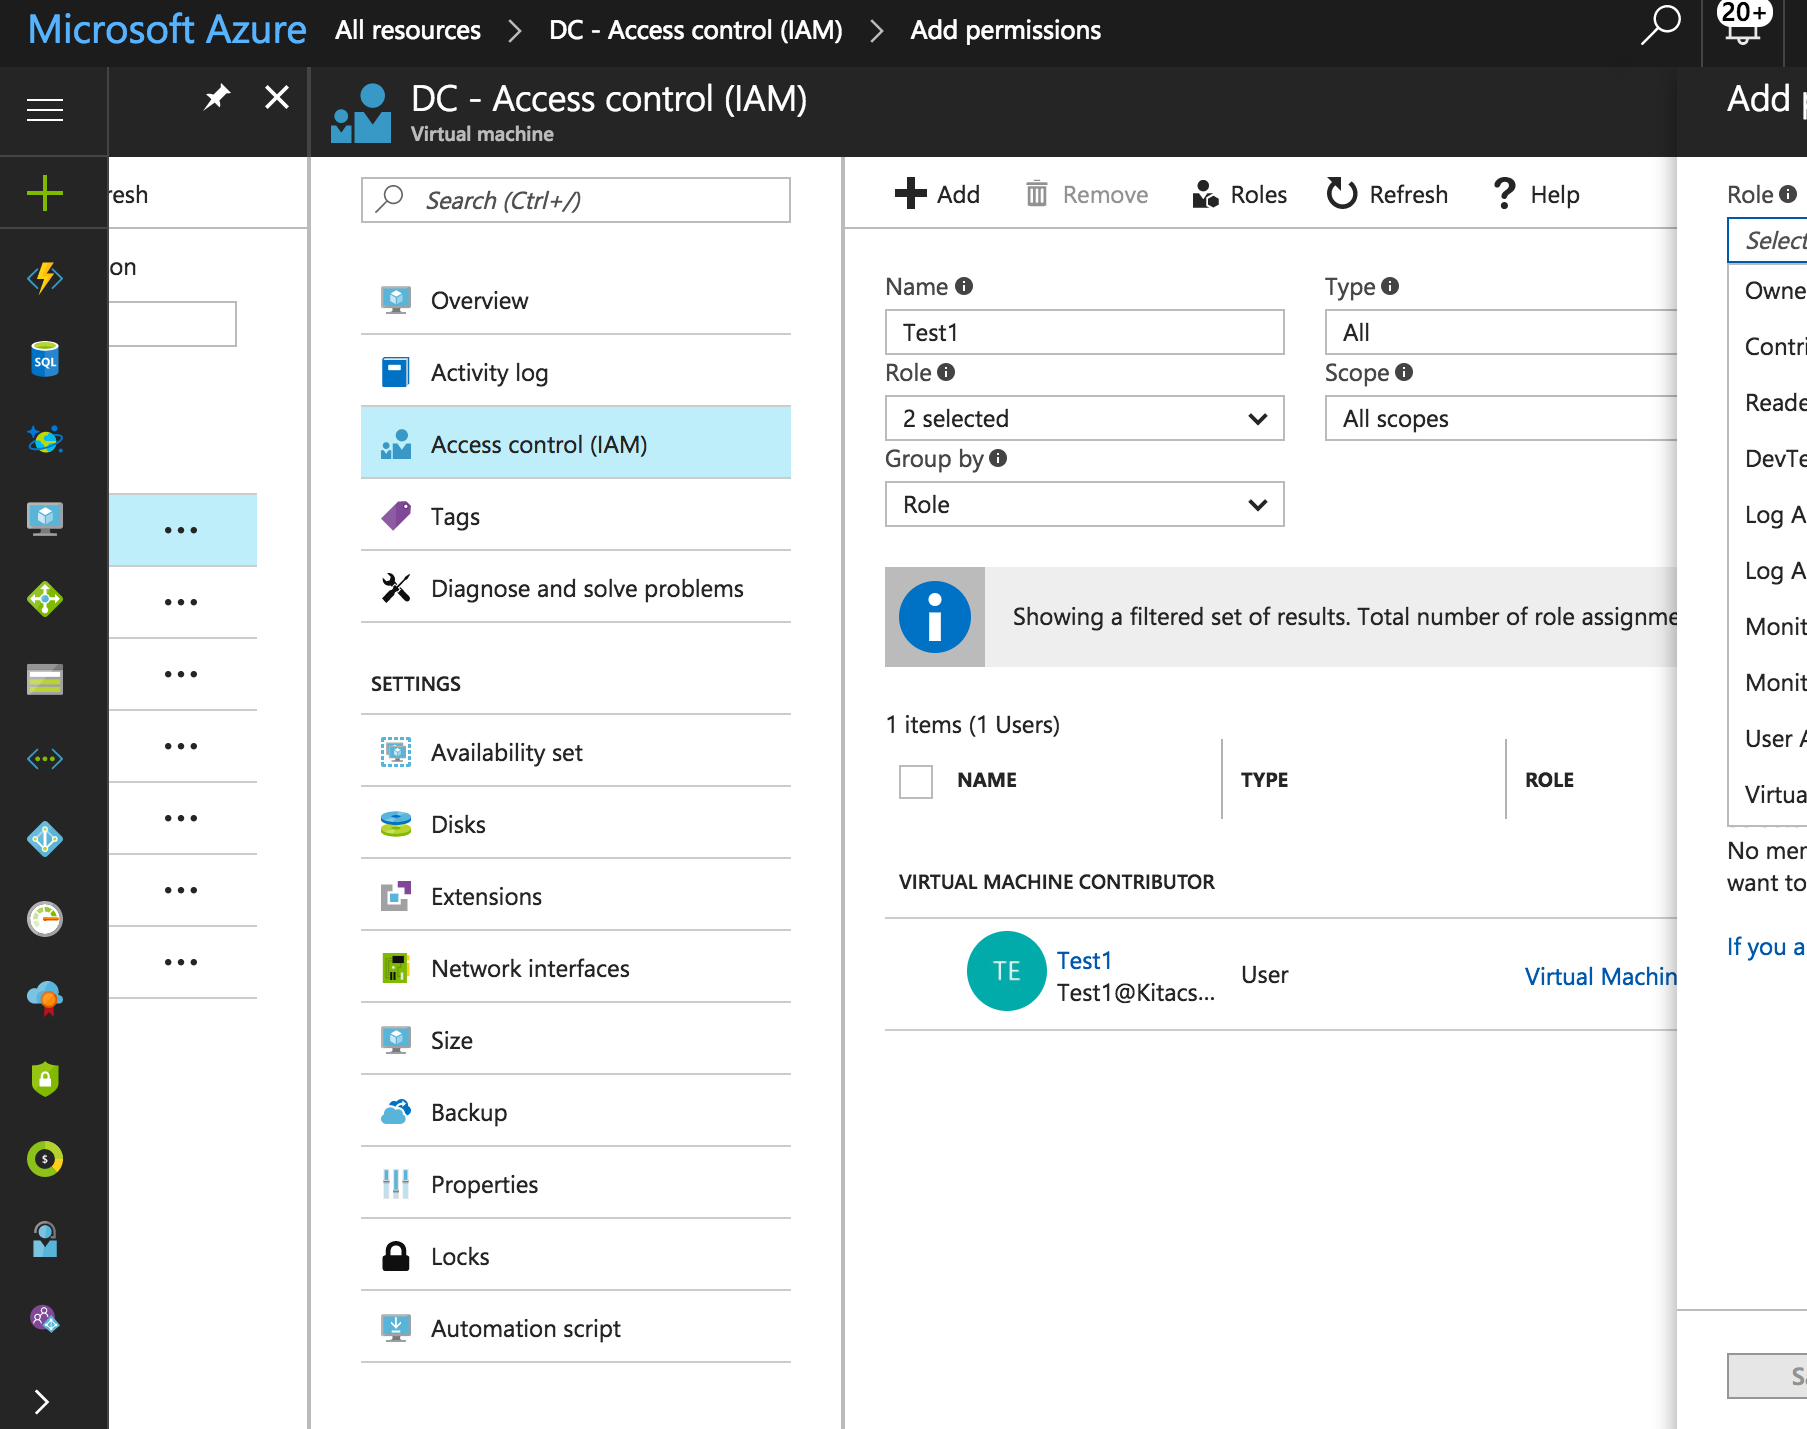
\includegraphics[width=0.8\textwidth]{res}
    \caption{Hinzufügen von Permissions.}
    \label{res}
\end{figure}

Zum Testen dienten die Benutzer. Vor der Zuweisung konnte sich der Benutzer am Virtual Machine nicht anmelden. Nachdem es diese Zuweisung durch die Rolle Leser beispielsweise gab, wurde die Virtual Machine DC als lesend im Azure-Portal aufgelistet und der Benutzer konnte auf die Ressource zugreifen. \\
\\
\section{Erstellen dynamischer Gruppen}
Dynamische Gruppen sind ein sehr hilfreiches Werkzeug, wenn es darum geht Benutzer dynamisch anhand von Attributen einer Gruppe zuzuordnen. Dabei kann man beispielsweise anhand seines Aufenthaltsort Zugriff auf bestimmte Ressourcen erlauben (wie es Beispielsweise bei Netflix der Fall ist). Oder Anhand einer Altersgruppe, können Zugangsbeschränkungen festgelegt werden, z.B.FSK18.
Zunächst muss dafür allerdings das Azure Premium Feature aktiviert werden, um auf die dynamische Gruppenverwaltung zuzugreifen. Dies geschieht wie folgt: Azure Active Directory > Licenses > All Products > try / buy > Activate Azure AD Premium. Als nächstes kann man dynamische Gruppen erstellen. Ich habe beispielhaft die vier Gruppen erstellt:
\\
\begin{itemize}
  \item DynamicTestGroup1: (user.userPrincipalName -startsWith "''Test"'') – Alle Benutzer, die im principal name „Test“-Anfang besitzen.
\item DynamicCountryGroup: (user.country -match "''Germany"'')-and(user.userPrincipalName -contains "''Kitacslab"'')
\item DynamicMailGroup: (user.userPrincipalName -contains "''Kitacslab"'')
\item DynamicJobGroup: (user.jobTitle -match "''SoftwareEngineer"'')
\end{itemize}


Regeln für eine bestimmte Gruppe können entweder einfach oder erweitert sein. Bei der einfachen Regel bekommt man eine vorgefertigte Maske mit definierten Mustern. Bei der erweiterten Regel lässt sich die Regel feingranularer mittels einer SQL-ähnlichen Syntax erstellen. Bei der Auflistung der Gruppen erkennt man eben diese Syntax
\begin{itemize}
  \item user.userPrincipalName -startsWith "'Test"') matcht auf allen Benutzern, die im Principal-Name mit „Test“-Anfangen
\item - (user.country -match "''Germany"')-and(user.userPrincipalName -contains "'Kitacslab"') – Alle Benutzer, die der Domain Kitacslab angehören und deren Land Deutschland ist
\item (user.jobTitle -match "'SoftwareEngineer"') sind alle Benutzer, die Software-Ingenieure sind.
\end{itemize}

\section{Row-Level Security}

Anhand der gegeben Viruellen Umgebung erarbeitet man Schritt für Schritt eine Row-Level-Security für einen neuen SQL-Server. Row-Level Security ist auf deutsch ganz einfach, Sicherheit auf Zeilenebene einer Datenbank und dient primär dazuden Zugriff auf Zeilen der Datenbanktabelle zu beschränken. Als Kriterium gelten auch hier wieder Attribute des Benutzers wie die Zugehörigkeit zu einem bestimmten Bereich (beispielsweise Bereich 3). Dabei steht vor allem im Vordergrund der authentifizierte Benutzer im sogenannten SESSION\_CONTEXT, in dem der aktuelle Benutzer, der auf eine Datenbank zugreift, gehalten wird. Man kann weiterhin auch Prädikaten zur Absicherung setzen, wie das FILTER und das BLOCK-Prädikat beispielsweise. Die gemäß ihres Namens entweder Zeilen filtern (wenn der Benutzer lesend zugreift oder blockieren (wenn der Benutzer schreibend zugreift). Tutorial wird auch sehr schnell bewusst, dass es sich bei den Operationen nur um Zugriffe auf Zeilen einer Datenbanktabelle handelt und nur auf die Zeilen zugreifen darf, die gemäß seines Attributes erlaubt sind. Greift ein Benutzer per Abfrage auf Daten der Datenbank zu, bekommt dieser zunächst nicht mit, dass Zeilen beispielsweise gefiltert wurden oder er für den Zugriff bestimmter Zeilen blockiert ist, da diese auch eventuell nicht existieren könnten und die Abfrage keine Filter auf Seiten des Benutzers enthält. Unautorisierter Zugriff ist somit nicht möglich, was ein sehr großer Vorteil ist, den Row-Level Security mitbringt. Ein Angreifer kann dies auch nicht manipulieren, da sich die Logik und die Prädikate im Backend des Servers befinden. Leider geschieht dies zu Lasten der Performanz, da Abfragen von mehreren Suchanfragen die Antwortzeit belasten wenn Zeilenweise zugegriffen wird ohne clientseitige Filter einzubauen. Eventuell versteht der Client die Antwort auch nicht: Ist er geblockt, oder gibt es gerade eine Störung bezüglich der Datenhaltung?

\section{Always Encrypted}
In diesen Kapitel wird ähnlich wie im Kapitel zuvor ein Tutorial über eine Virtuelle Maschine durchgearbeitet. Das Microsoft Azure Feature namens „Always Encrypted“ dient zum Schutz von vertraulichen Daten in SQL-Datenbanken und zur Speicherung von Schlüsseln, die zur Verschlüsselung verwendet wurden, im sogenannten Windows-Zertifikatspeicher (\url{https://docs.microsoft.com/de-de/azure/sql-database/sql-database-always-encrypted}).
Das Prinzip, das dahinter steckt ist, dass Daten, die auf einem Server abgelegt sind, beim Austausch zwischen Server und Cleint nicht von dritten unverschlüsselt abgefangen werden können. Somit wird das Schutzziel Vertraulichkeit umgesetzt. Vor der Man-in-the-Middle-Attacke der Datenaustausch zumindest geschützt. Wurde eine Ressource verschlüsselt, kann diese nur von einem Client entschlüsselt werden, der Zugriff auf den Schlüssel zur Entschlüsselung besitzt.\\
Im Tutorial wird das Feature ebenfalls wieder für eine SQL-Datenbank konfiguriert. In dem Tutorial wird demonstriert, wie das Feature angewendet wird und die Datenbank in eine Beispielanwendung eingebunden werden kann. Geleitet wird man durch den \texttt{Always Encryptet Wizard}, der einen Schritt für Schritt zur Verschlüsselung von Datenbanktabellenspalten führt. Für die Verschlüsselung dieser Spalten werden sogenannte \texttt{Column Encryption Keys (CEK)} verwendet. Die CEKs selber müssen durch einen \texttt{Column Master Key} verschlüsselt werden, der auf dem Windows-Zertifikatspeicher abgelegt ist.\\
Abschließend wird im Tutorial gezeigt, wie der Einsatz des \texttt{Always Encrypted}-Feature mithilfe einer Anwendung erfolgt. Dabei wird die Datenbank in der Anwendung eingebunden und Daten hinzugefügt oder abgerufen.
\\
Das \texttt{Always Encrypted}-Feature schützt, wie bereits erwähnt, Hauptsächlich vor dem unerlaubten Zugriff und Lesen von Daten, indem das Schutzziel Vertraulichkeit umgesetzt wird. Fehlt dem Angreifer nämlich der \texttt{Column Master Key} oder CEK, kann dieser mit den verschlüsselten Daten nichts anfangen.
Die Performanz leidet bei diesem Feature überhaupt nicht, da die Daten mittels Schlüssel ver- und entschlüsselt werden können, was keinen großen Verlust seitens der Performanz einbringt.

Zusammenfassung

Zusammenfassend lässt sich sagen, dass \texttt{Row-Level}-Security für die Sicherheit des unerlaubten Zugriffs anhand von Attributen auf Zeilenebene zuständig ist und \texttt{Always Encrypted}-Feature die Spalten einer Datenbanktabelle verschlüsselt. Somit bieten beide unterschiedliche Eigenschaften, um den Zugriff auf Daten einer Datenbank zu schützen. RLS dient hauptsächlich für eine Vielzahl von Consumer, da dort sehr gut gefiltert werden kann, was wer wie sehen darf. Wohingegen \texttt{Always Encrypted} für den Gebrauch von Austausch sensibler Daten zwischen Client und Server dient.

\docend
%%% end of document
